\section{Results}


\subsection{Correlations with exogenous variables}

The results of calibrating our model are encouraging as we find high correlations between the results of our $w^*_e$ algorithm and our exogenous variables $v$. 

We define $\rho$ at the maximum achievable spearman rank correlation between $w^*$ and $v$ for editors or articles, by category, and over time. The variation of $\rho$, by for editor for any category ranges from 0.75 to 0.46 with a mean 0.64.  That same statistic for articles is articles from 0.91 to 0.57 with a mean of 0.72, which is overall higher.

 
From snapshotting we see view $\rho$ as  a function of time. In the case of editors we see increasing trends in all categories over time. This means that $w^*_e$ benefits from incorporating more contribution history. As for articles, from the start of a category's history the correlations remain stable. \ref{fig:rhotime}

\begin{figure}[!t]
\centering
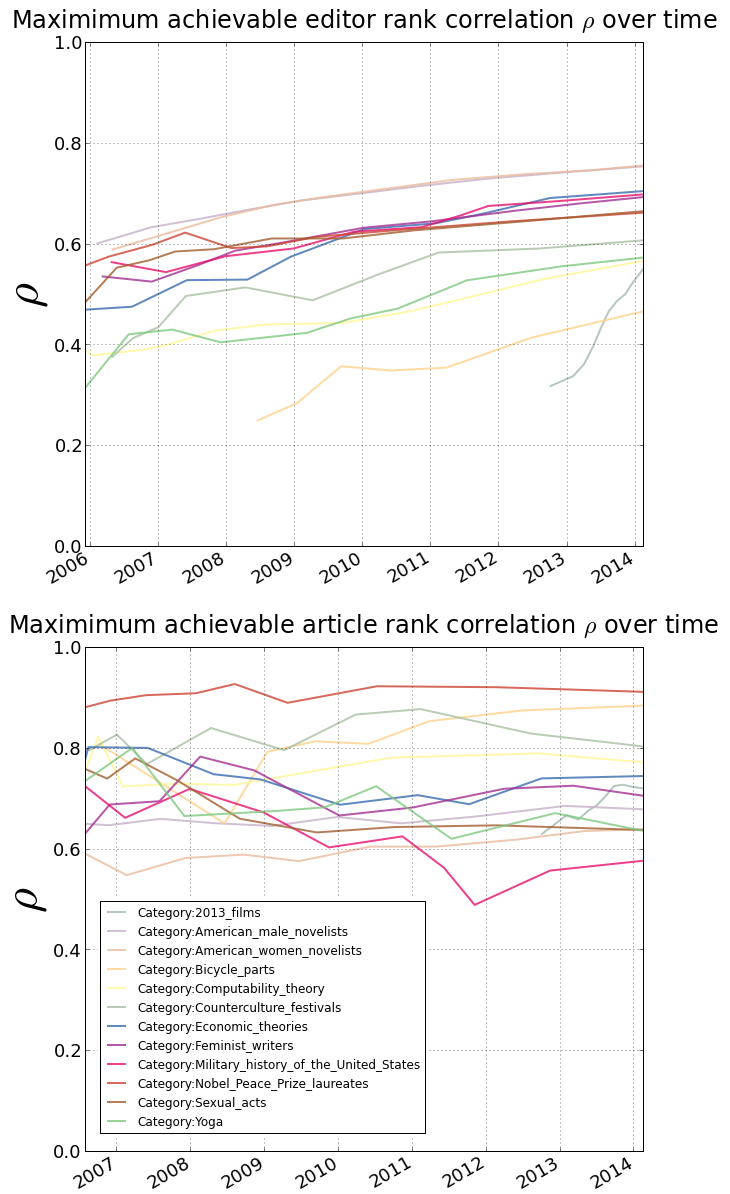
\includegraphics[width=0.9\columnwidth]{rho_combined.png}.
\caption{$\rho$ over time, by category and type}
\label{fig:rhotime}
\end{figure}


%$\alpha$ is a measure of how important it is for quality that many users edit, with lower alpha, we have a more collaborative category, where edits are more equal and egalitarean. With alpha high, the category is more rewarding users that operate more individualistically. Beta is inversely related to alpha so the same can be said but the directions of the arguments reversed. This means we can talk of the characteristic of a category, compared to one another and compared over time. 

\subsection{Negative values of $\alpha$ and $\beta$}
Another surprising result is that we find at times, negative values for $\alpha$ and $\beta$.


For editors, maximum $\rho$ always occurs strictly within a radius of 0.01 around the origin on the  $\alpha$-$\beta$ plane. The $(0,0)$ solution is significant in that it represents unbiased arithmetic averages.
\ref{fig:landscape}

For articles, the solutions have varied solutions, possibly including a negative alpha. For instance in Category Economic Theories we find a family of maximizing solutions with a negative values of $\alpha$ and $\beta$. \ref{fig:landscape} Why there should be this family is due optimizing solutions is due to a number of reasons. One is our use of the ranking correlation. Since we are comparing only ranks positions, there are many ways to achieve our best-prediction list and perturbing $\alpha$ and $\beta$ do not affect the rank being produced. This also means that the behaviour displayed by the  landscape indicates that one of several possibilities: That either $\alpha$ is positive but small, in which case $\beta$ is bounded tightly, which means that better editors are producing more obscure articles. Or that $\alpha$ is negative and that $\beta$ is more loosely bounded. This indicates that $\alpha$ is dominating, as is the case in equations (2). In our particular example we also find that this family is shifted towards the positive $\beta$ axis. So even as the trade off occurs, its favours $\beta$ which interpreted through equations (2) means that editors who edit relatively more obscure articles are important to success of articles in Category Economic Theories.
%move to discussionIf $\alpha$ show the importance of the fittest editors contributing, negative alpha goes to imply that in these cases its actually important that less fit editors contribute at these points. This shows anti-competetiveness. Negative beta would mean that for an editor the production of ubiquitious, common, heavily otherwise-edited articles are important. Which again is a reward for anti-competitive behaviour.

\begin{figure}[!t]
\centering
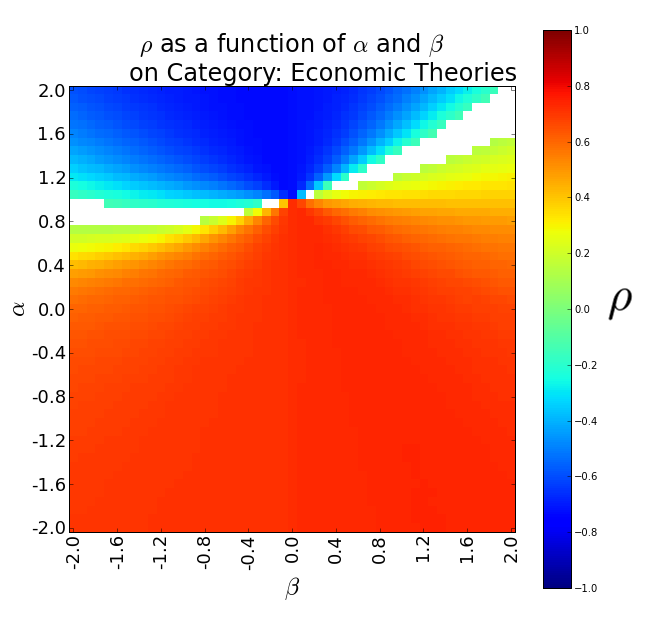
\includegraphics[width=0.9\columnwidth]{landscape.png}.
\caption{Landscape}
\label{fig:landscape}
\end{figure}

